\documentclass[a4paper,12pt]{article} % тип документа

%  Русский язык
\usepackage[T2A]{fontenc}			% кодировка
\usepackage[utf8]{inputenc}			% кодировка исходного текста
\usepackage[english,russian]{babel}	% локализация и переносы

\usepackage{graphicx, scalerel}               % импорт изображений
\usepackage{wrapfig}                % обтекаемые изображения
\graphicspath{{pictures/}}          % обращение к подкаталогу с изображениями
\usepackage[14pt]{extsizes}         % для того чтобы задать нестандартный 14-ый размер шрифта
\usepackage[warn]{mathtext}         % русский язык в формулах
\usepackage{indentfirst}            % indent first
\usepackage[margin = 25mm]{geometry}% отступы полей
\usepackage[table,xcdraw]{xcolor}   % таблицы
\usepackage{amsmath,amsfonts,amssymb,amsthm,mathtools} % Математика
\usepackage{wasysym}                % ???
\usepackage{upgreek}                % ???  
\usepackage{caption}
\usepackage{multirow}
\captionsetup{labelsep=period}
\usepackage[font=small,labelfont=bf]{caption}
\usepackage{gensymb} % degree symbol
\usepackage{tikz}
\usetikzlibrary{positioning}


\begin{document}
	
	
	\begin{center}
		
		
		\textbf{НАЦИОНАЛЬНЫЙ ИССЛЕДОВАТЕЛЬСКИЙ УНИВЕРСИТЕТ \\ <<МОСКОВСКИЙ ФИЗИКО-ТЕХНИЧЕСКИЙ ИНСТИТУТ>>}
		\vspace{13ex}
		
		\textbf{Лабораторная работа 4.3.2\\ <<Дифракция света на ультразвуковой волне в жидкости \\ (Горизонтальная щель)>>}
		\vspace{40ex}
		
		\normalsize{Овсянников Михаил Александрович \\ студент группы Б01-001\\ 2 курс ФРКТ\\}
	\end{center}
	
	\vfill 
	
	\begin{center}
		г. Долгопрудный\\ 
		2022 г.
	\end{center}
	
	
	\thispagestyle{empty} % выключаем отображение номера для этой страницы
	\newpage
	
	
	\textbf{Цель работы:} изучение дифракции света на синусоидальной акустической решетке и наблюдение фазовой решетки методом темного поля.
	
	\textbf{В работе используются:} оптическая скамья, осветитель, два длиннофокусных объектива, кювета с жидкостью, кварцевый излучатель с микрометрическим винтом, генератор звуковой частоты, линза, вертикальная нить на рейтере, микроскоп.
	
	
	
	
	\section*{Теоретические сведения}

	
	При прохождении ультразвуковой волны через жидкость в ней возникают периодические неоднородности коэффициента преломления, создается фазовая решетка, которую мы считаем неподвижной ввиду малости скорости звука относительно скорости света. Показатель
	преломления n изменяется по закону:
	
	\begin{equation*}
		n = n_0 (1 + m \cos \Omega x)
	\end{equation*}
	
	Здесь $ \Omega = 2 \pi / \Lambda $ --- волновое число для ультразвуковой волны, $ m $ --- глубина модуляции $ n $ $ (m \ll 1 $).
	
	Положим фазу $ \phi $ колебаний световой волны на передней стенке кюветы равной нулю, тогда на задней поверхности она равна:
	
	\begin{equation*}
		\varphi  = k n L = \varphi_0 (1 + m \cos \Omega x)
	\end{equation*}
	
	Здесь $ L $ --- толщина жидкости в кювете, $ k = 2 \pi / \lambda $ --- волновое число для света.
	
	После прохождения через кювету световое поле есть совокупность плоских волн, распространяющихся под углами $ \theta $, соответствующими максимумам в дифракции Фраунгофера:
	
	\begin{equation*}	
		\Lambda \sin \theta_m = m \lambda
	\end{equation*}
	
	Этот эффект проиллюстрирован на рисунке 1.
	\begin{figure}[h!]
		\centering	
		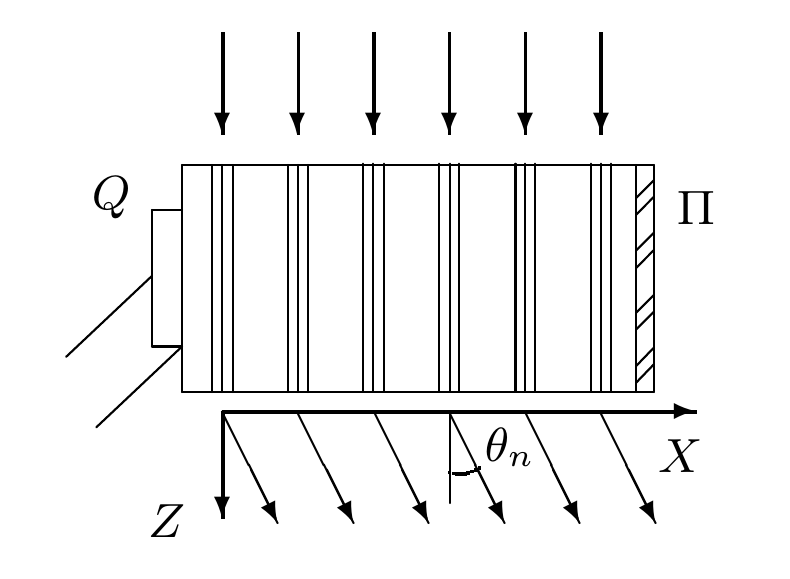
\includegraphics[width=0.4\textwidth]{Pictures/image_1}
		\caption{Дифракция световых волн на акустической решетке}
		\label{diff}
	\end{figure}
	
	Зная положение дифракционных максимумов, легко определить длину ультразвуковой волны, учитывая малость $ \theta $: $ \sin \theta \approx \theta \approx l_m /F  $, где $ l_m $ --- расстояние от нулевого до последнего видимого максимума, $ F $ --- фокусное расстояние линзы. Тогда получим:
	
	\begin{equation*}
		\Lambda = m \lambda F/ l_m 
	\end{equation*}
	Скорость ультразвуковых волн в жидкости, где $ \nu $ --- частота колебаний излучателя:
	
	\begin{equation*}
		v = \Lambda \nu 
	\end{equation*}
	
	\section*{Экспериментальная установка}
	
	Схема установки приведена на рисунке 2. Источник света Л через светофильтр Ф и конденсор К освещает вертикальную щель $ S $, находящуюся в фокусе объектива $ O_1 $. После объектива параллельный световой пучок проходит через кювету С перпендикулярно акустической решетке, и дифракционная картина собирается в фокальной плоскости объектива $ O_2 $ , наблюдается при помощи микроскопа $M$.
	
	Предварительную настройку установки произведем в соответствии с инструкцией с зеленым фильтром, далее в работе используется красный.
	
	\begin{figure}[h!]
		\centering	
		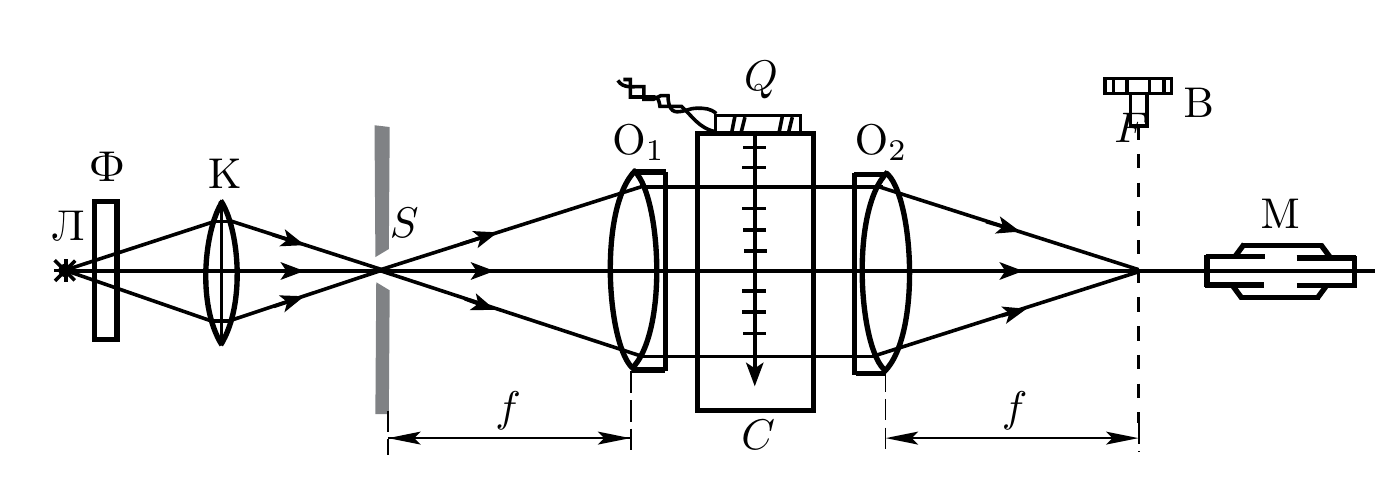
\includegraphics[width=0.9\textwidth]{Pictures/image_2}
		\caption{Схема для наблюдения дифракции на акустической решетке}
		\label{shema1}
	\end{figure}
	
	Фокусное расстояние объектива $ O_2$: $F = 28 $ см, цена деления винта микроскопа -- 4 мкм, погрешность измерений примем равной  $ \sigma = $ 1 деление, или 4 мкм. Полоса пропускания фильтра $ \lambda = 6400 \pm 200$ \AA.
	
	\newpage
	
	\section*{Ход работы}
	
	\begin{center}
		\textbf{I. Определение скорости ультразвука по дифракционной картине}
	\end{center}

	\begin{enumerate}
		\item Соберем схему согласно рисунку. Отцентрируем систему и установим ширину щели равной 25 мкм.
		
		\item Получим дифракционную картину.
		
		Перемещая излучатель с помощью лимба, оценим по порядку величины длину УЗ волны как удвоенное расстояние между наиболее четкими картинами: $\Lambda = 2 \cdot 53 \text{ дел}\cdot 10\frac{\text{мкм}}{\text{дел}} = 1,06$ мм.
		
		\item Определим положения дифракционных полос. С помощью перекрестия и микрометрического винта, установленного на выходе прибора, определим координату $Y$ каждой светлой полосы в делениях винта. 
		
		Проделаем данную операцию для трех частот. Результаты занесем в таблицу 1.
		
		\begin{table}[h!]
			\centering
				\begin{tabular}{|cc|cccclccc}
					\cline{1-2} \cline{5-6} \cline{9-10}
					\multicolumn{1}{|c|}{$m$}  & $Y$, дел &  & \multicolumn{1}{c|}{} & \multicolumn{1}{c|}{$m$} & \multicolumn{1}{c|}{$Y$, дел} &  & \multicolumn{1}{c|}{} & \multicolumn{1}{c|}{$m$} & \multicolumn{1}{c|}{$Y$, дел} \\ \cline{1-2} \cline{5-6} \cline{9-10} 
					\multicolumn{2}{|c|}{$\nu = 1,044$ МГц} &  & \multicolumn{1}{c|}{} & \multicolumn{2}{c|}{$\nu = 1,504$ МГц}                     &  & \multicolumn{1}{c|}{} & \multicolumn{2}{c|}{$\nu = 2,014$ МГц}                     \\ \cline{1-2} \cline{5-6} \cline{9-10} 
					\multicolumn{1}{|c|}{-4}   & -127     &  & \multicolumn{1}{c|}{} & \multicolumn{1}{c|}{-2}  & \multicolumn{1}{c|}{-80}      &  & \multicolumn{1}{c|}{} & \multicolumn{1}{c|}{-1}  & \multicolumn{1}{c|}{-64}      \\ \cline{1-2} \cline{5-6} \cline{9-10} 
					\multicolumn{1}{|c|}{-3}   & -93      &  & \multicolumn{1}{c|}{} & \multicolumn{1}{c|}{-1}  & \multicolumn{1}{c|}{-45}      &  & \multicolumn{1}{c|}{} & \multicolumn{1}{c|}{0}   & \multicolumn{1}{c|}{0}        \\ \cline{1-2} \cline{5-6} \cline{9-10} 
					\multicolumn{1}{|c|}{-2}   & -65      &  & \multicolumn{1}{c|}{} & \multicolumn{1}{c|}{0}   & \multicolumn{1}{c|}{0}        &  & \multicolumn{1}{c|}{} & \multicolumn{1}{c|}{1}   & \multicolumn{1}{c|}{71}       \\ \cline{1-2} \cline{5-6} \cline{9-10} 
					\multicolumn{1}{|c|}{-1}   & -34      &  & \multicolumn{1}{c|}{} & \multicolumn{1}{c|}{1}   & \multicolumn{1}{c|}{43}       &  &                       &                          &                               \\ \cline{1-2} \cline{5-6}
					\multicolumn{1}{|c|}{0}    & 0        &  & \multicolumn{1}{c|}{} & \multicolumn{1}{c|}{2}   & \multicolumn{1}{c|}{85}       &  &                       &                          &                               \\ \cline{1-2} \cline{5-6}
					\multicolumn{1}{|c|}{1}    & 31       &  &                       &                          &                               &  &                       &                          &                               \\ \cline{1-2}
					\multicolumn{1}{|c|}{2}    & 69       &  &                       &                          &                               &  &                       &                          &                               \\ \cline{1-2}
					\multicolumn{1}{|c|}{3}    & 104      &  &                       &                          &                               &  &                       &                          &                               \\ \cline{1-2}
					\multicolumn{1}{|c|}{4}    & 139      &  &                       &                          &                               &  &                       &                          &                               \\ \cline{1-2}
				\end{tabular}
			\caption{Результаты измерений}
		\end{table}
		
		\item Построим на одном листе графики $Y = Y(m)$ для каждой частоты. Все на графике 1.
		\newpage
		\begin{figure}[h!]
			\centering
			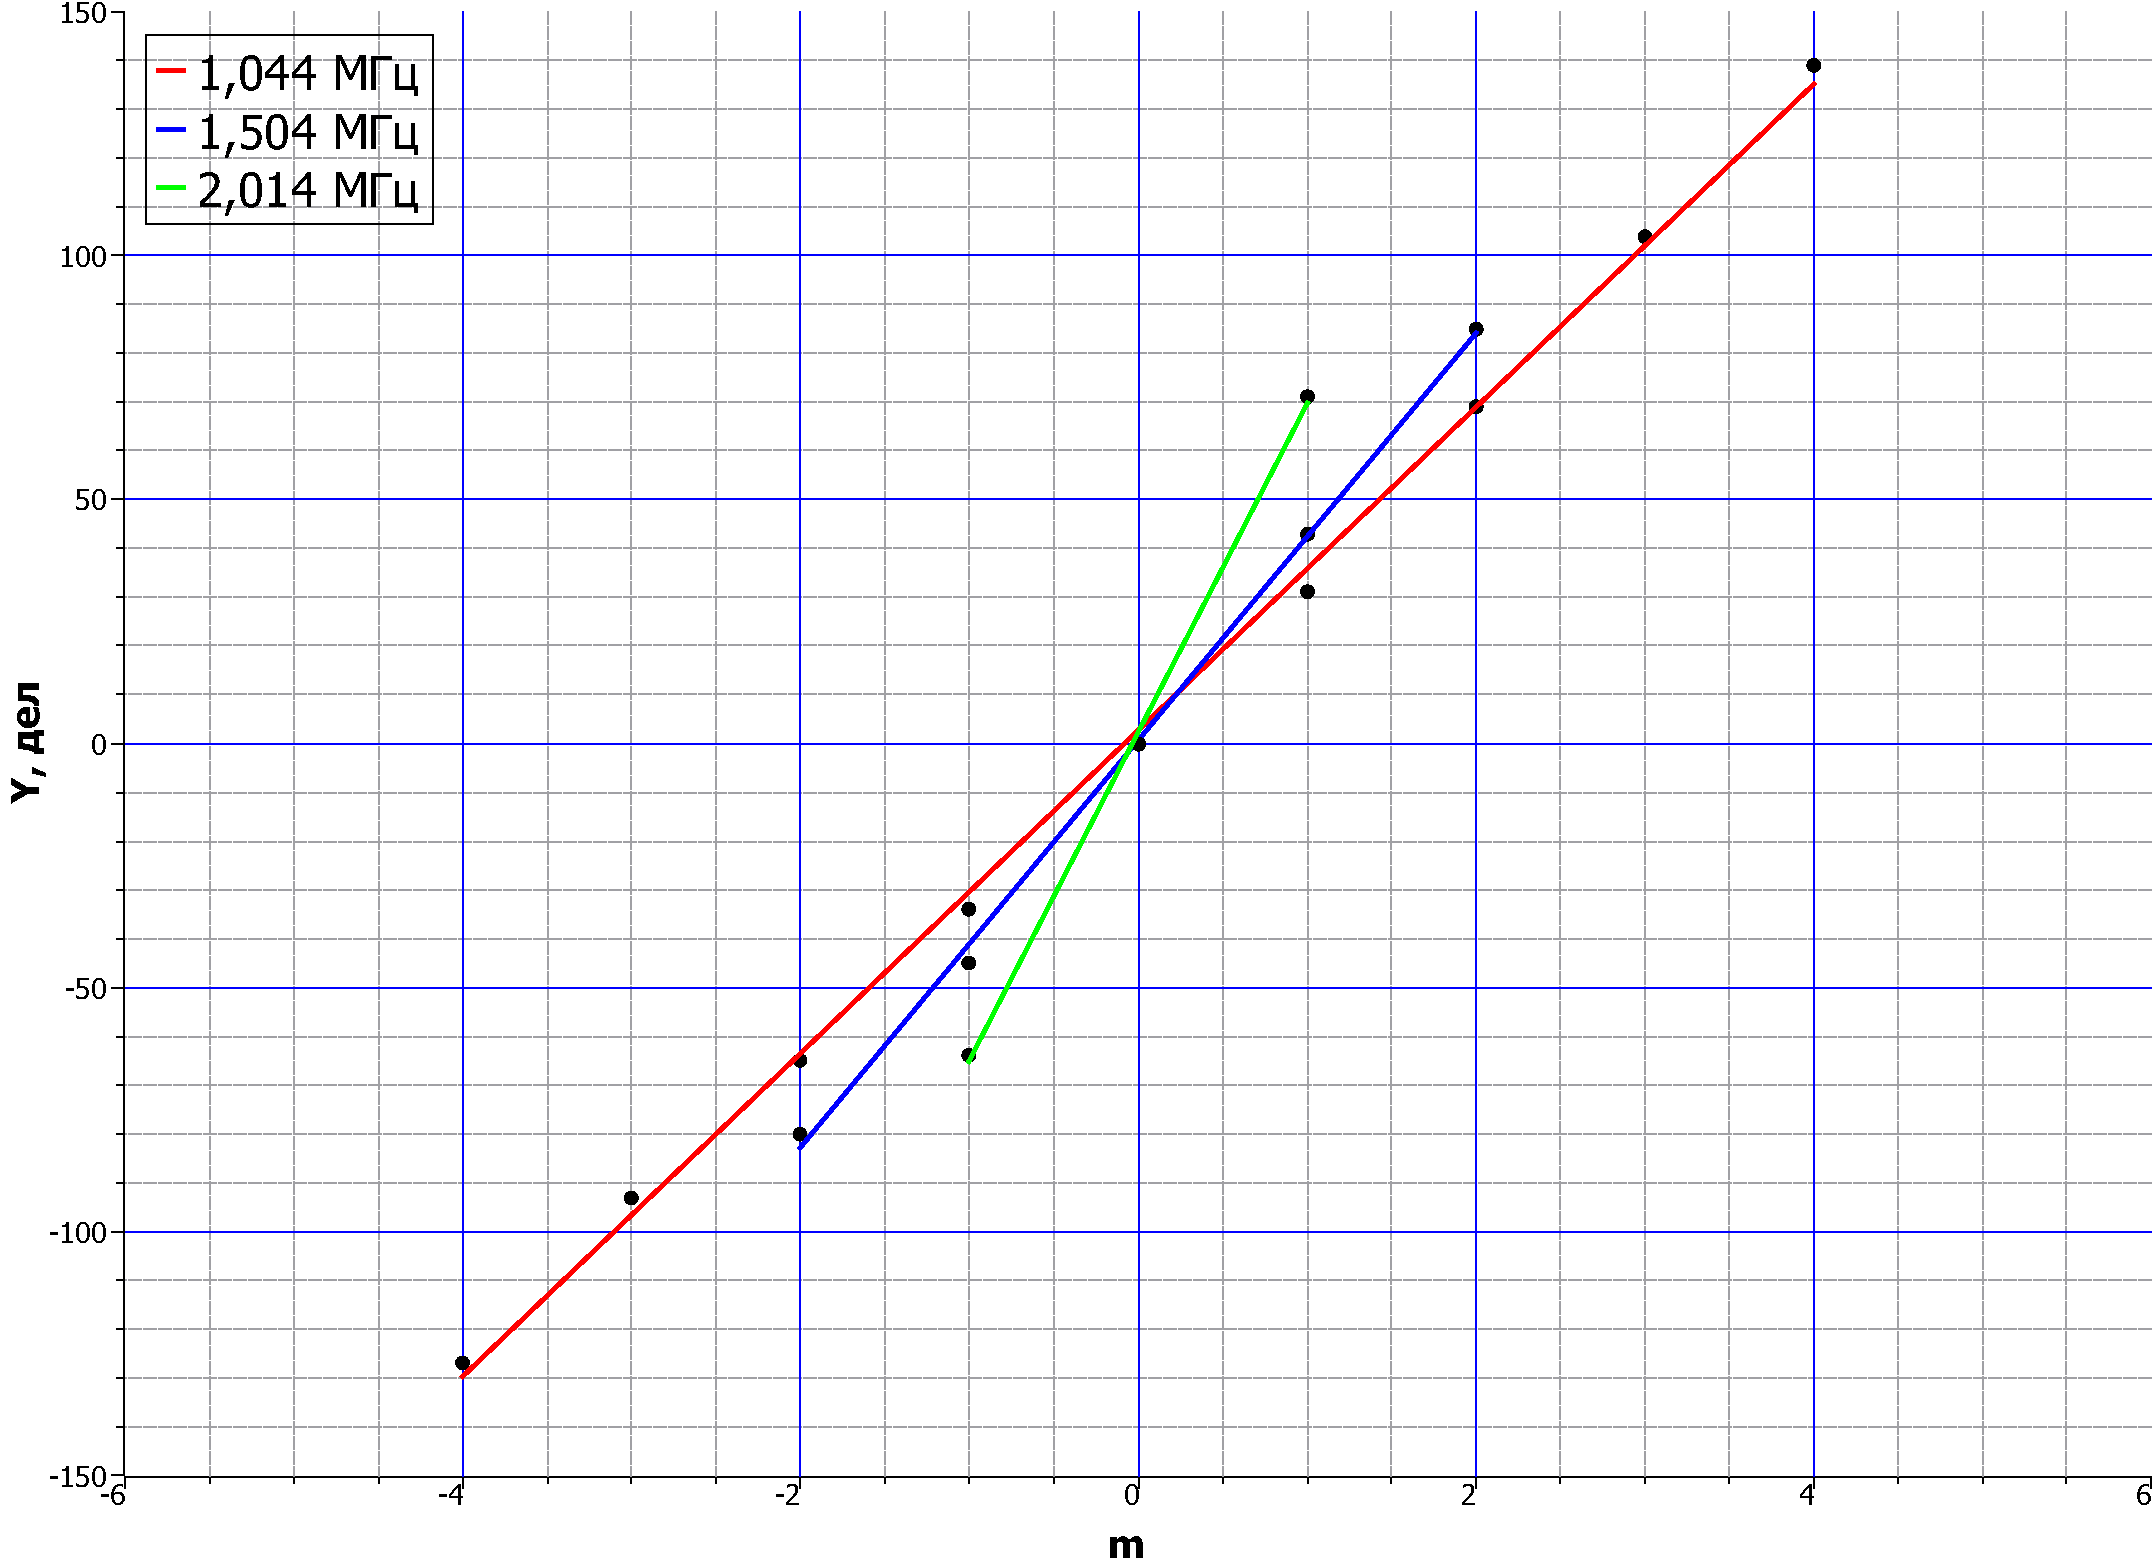
\includegraphics[width=0.9\linewidth]{Pictures/Graphs}
			\caption{Зависимость $Y(m)$ для разных частот}
		\end{figure}
	
	Для прямых на рисунке получаем коэффициенты наклона:
	
	$\boxed{k_1 = (33,1 \pm 0,5) \text{ дел}} \;\;\;\; \boxed{k_2 = (41,8 \pm 0,9) \text{ дел}} \;\;\;\; \boxed{k_3 = (68 \pm 2) \text{ дел}}$
	
	\item Рассчитаем длину УЗ-волны и скорость звука для каждой частоты.
	\begin{equation*}
		\Lambda = \frac{mf\lambda}{l_m} \hspace{30mm} v = \Lambda\nu
	\end{equation*}

	\begin{table}[h!]
		\centering
		\begin{tabular}{|cc|}
			\hline
			\multicolumn{2}{|c|}{$\nu$, 1,044 МГц}                \\ \hline
			\multicolumn{1}{|c|}{$\Lambda$, мм} & 1,36 $\pm$ 0,05 \\ \hline
			\multicolumn{1}{|c|}{$v$, м/с}      & 1420 $\pm$ 50   \\ \hline
			\multicolumn{2}{|c|}{$\nu$, 1,504 МГц}                \\ \hline
			\multicolumn{1}{|c|}{$\Lambda$, мм} & 1,09 $\pm$ 0,04 \\ \hline
			\multicolumn{1}{|c|}{$v$, м/с}      & 1640 $\pm$ 60   \\ \hline
			\multicolumn{2}{|c|}{$\nu$, 2,014 МГц}                \\ \hline
			\multicolumn{1}{|c|}{$\Lambda$, мм} & 0,66 $\pm$ 0,03 \\ \hline
			\multicolumn{1}{|c|}{$v$, м/с}      & 1330 $\pm$ 60   \\ \hline
		\end{tabular}
		\caption{Обработанные результаты}
	\end{table}

	Как видно, результаты достаточно близки друг к другу и почти совпадают с табличными значениями: $v = 1500$ м/с.
		
	\end{enumerate}

	\newpage
	
	\begin{center}
		\textbf{II. Определение скорости ультразвука методом темного поля}
	\end{center}

	\begin{enumerate}
		\item Для перехода к методу темного поля отодвинем микроскоп от щели и разместим в промежутке между ними дополнительную линзу.
		
		Поднимем излучатель над кюветой и опустим в воду квадратную сетку. Отцентрируем систему, чтобы сетку было четко видно в микроскопе. Рассчитаем цену деления в этом эксперименте, зная, что размер квадратика сетки 1 мм. Получаем $\boxed{0,14 \frac{\text{мм}}{\text{дел}}}$
		
		
		\item Установим ширину щели 25 мкм. Уберем калибровочную сетки и опустим излучатель. Постараемся увидеть звуковую решетку.
		
		\item Закроем нулевой дифракционный максимум проволочкой. Поле зрения микроскопа затемняется.
		
		\item Меняя частоту, будем наблюдать акустическую решетку.
		
		\item Зафиксируем с помощью окулярной шкалы микроскопа координаты первой и последней из хорошо видимых темных полос и количество светлых промежутков между ними. Проделаем это для 4 разных частот. Результаты пишем в таблицу 3.
		
		\begin{table}[h!]
			\centering
			\begin{tabular}{|c|c|c|c|}
				\hline
				$\nu$, МГц & \begin{tabular}[c]{@{}c@{}}Координата\\ верхней полосы\end{tabular} & \begin{tabular}[c]{@{}c@{}}Координата\\ нижней полосы\end{tabular} & \begin{tabular}[c]{@{}c@{}}Количество\\ светлых полос\end{tabular} \\ \hline
				1,0056     & 60                                                                  & 0,0                                                                 & 12                                                                 \\ \hline
				1,1900     & 68                                                                  & 0,0                                                                & 20                                                                 \\ \hline
				1,3700     & 53                                                                  & 0,1                                                                & 14                                                                 \\ \hline
				1,6500     & 67                                                                  & 0,0                                                                 & 20                                                                 \\ \hline
			\end{tabular}
			\caption{Результаты}
		\end{table}
		
		
		\item Для каждой частоты рассчитаем длину $\Lambda$ УЗ-волны.
		Посчитанные значения заносим в таблицу 4.
		\begin{table}[h!]
			\centering
			\begin{tabular}{|c|c|}
				\hline
				$\nu$, МГц & $\Lambda$, мм \\ \hline
				1,0056     & 1,412         \\ \hline
				1,1900     & 1,190         \\ \hline
				1,3700     & 1,060         \\ \hline
				1,6500     & 0,938         \\ \hline
			\end{tabular}
			\caption{Зависимость длины волны от частоты}
		\end{table}
		
		\newpage		
		
		\item Построим график зависимости $\Lambda (1/\nu)$.
		
		\begin{figure}[h!]
			\centering
			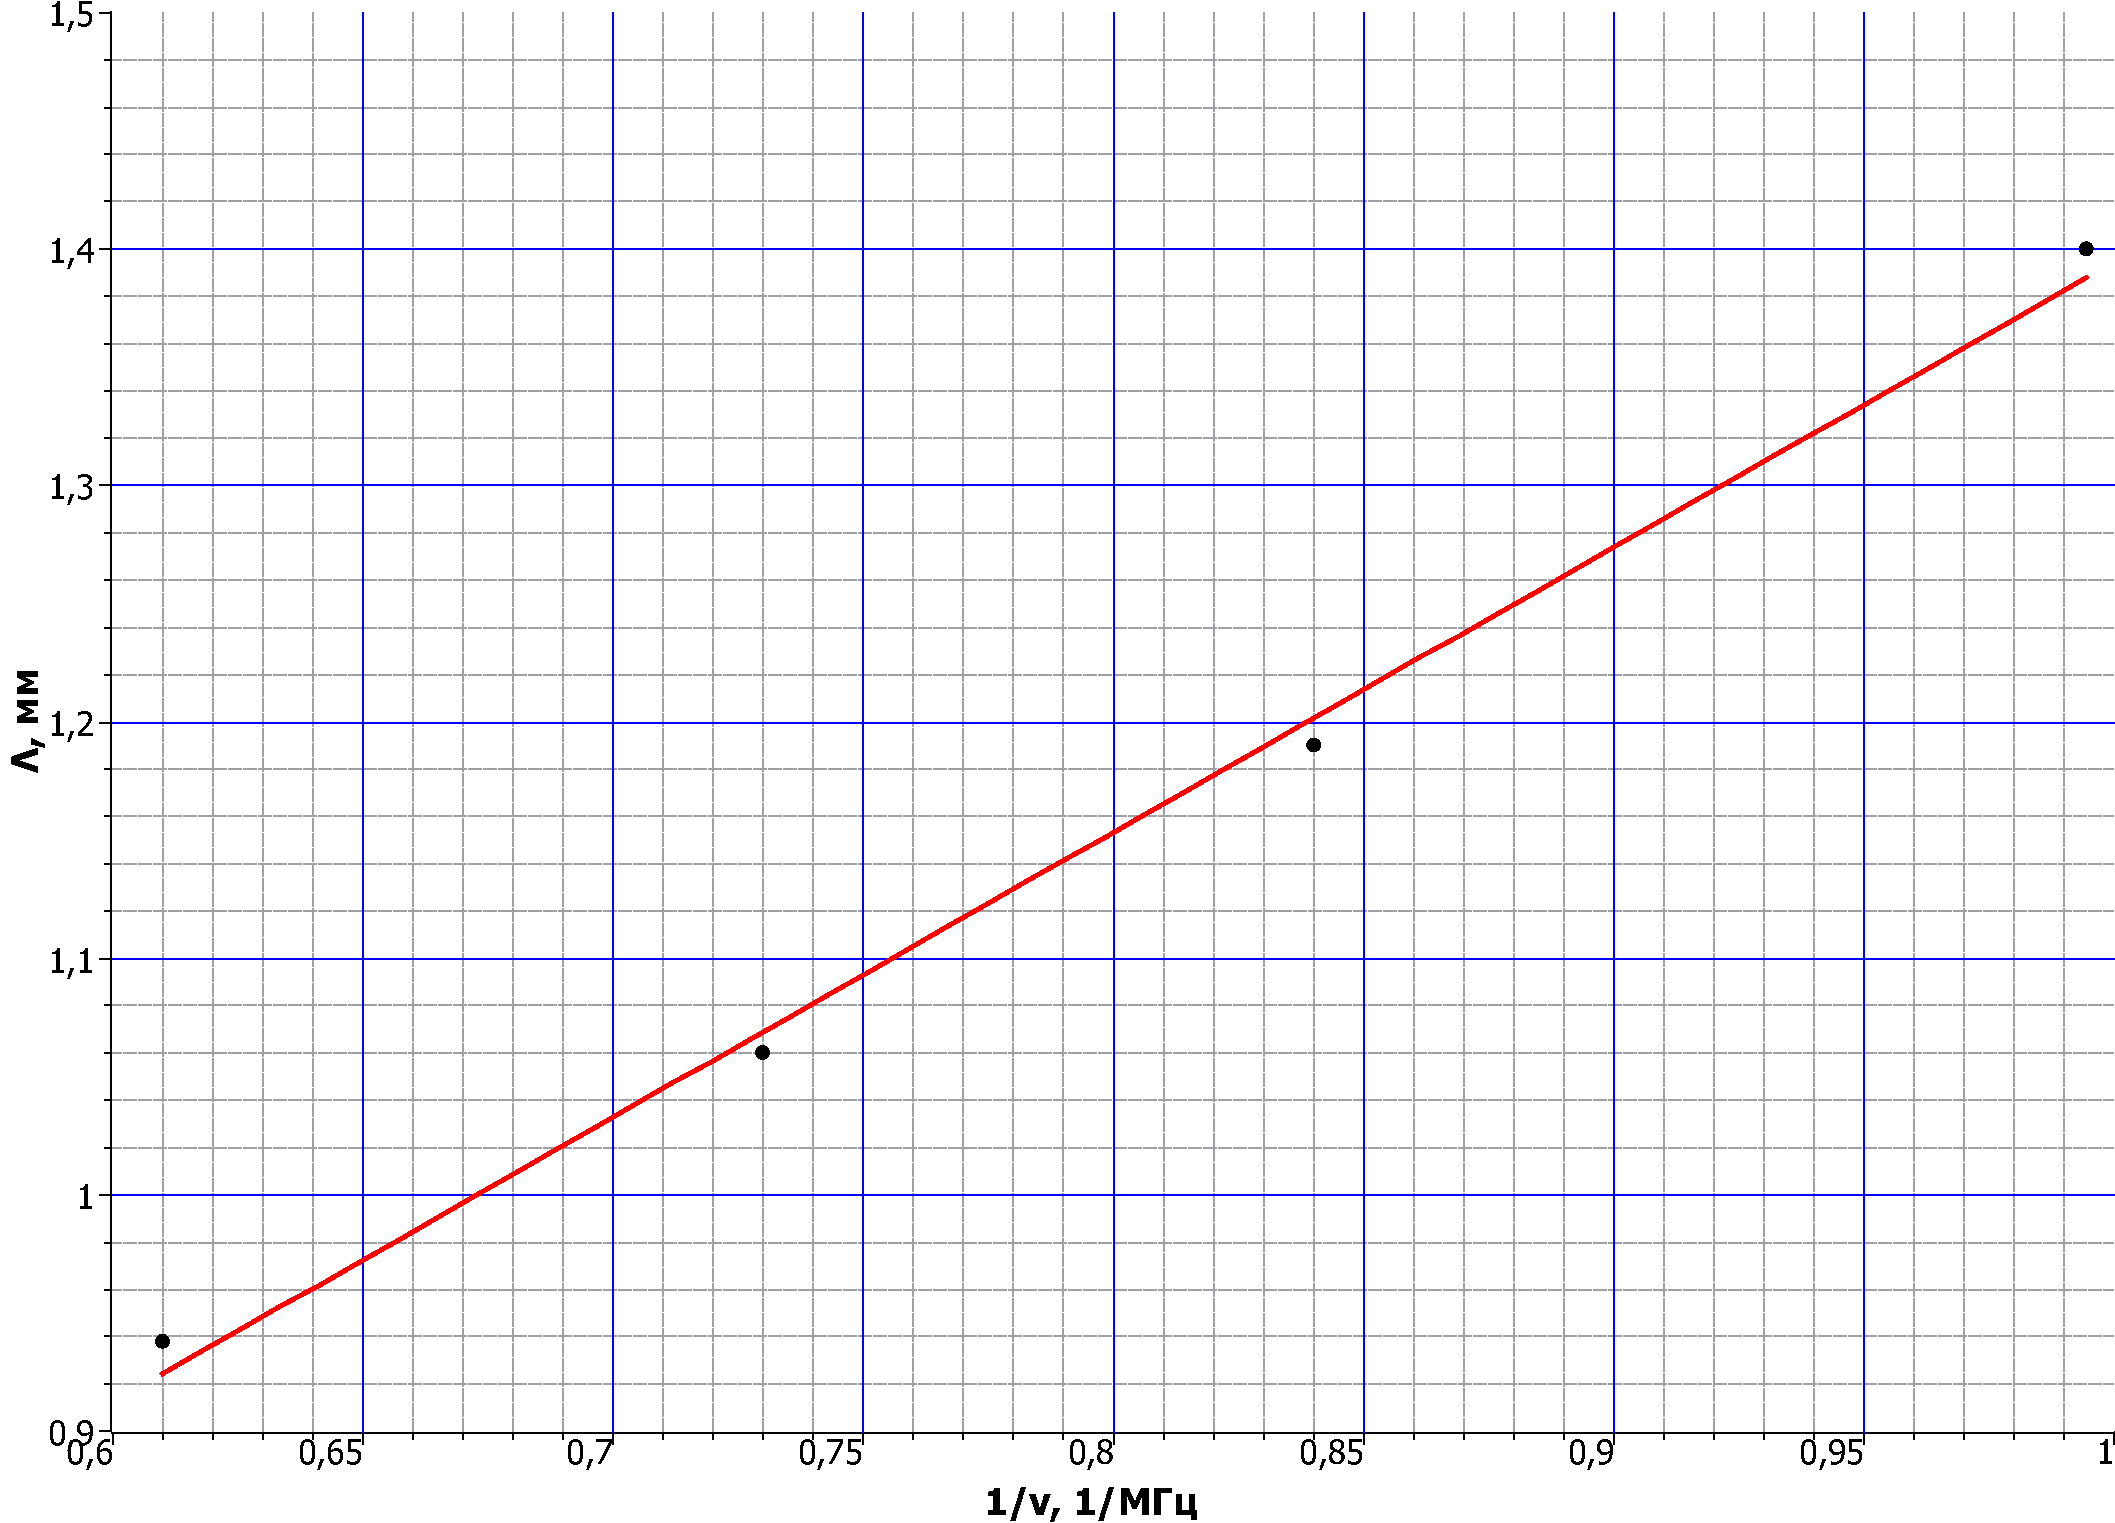
\includegraphics[width=0.9\linewidth]{Pictures/Lambda(nu)}
			\caption{График зависимости $\Lambda (1/\nu)$}
		\end{figure}
		
		По наклону определим скорость ультразвука.
		\begin{equation*}
			v = \Lambda \nu = k = (1,46 \pm 0,09) \; \text{мм} \cdot \text{МГц} = (1460 \pm 90 \; \text{м/с}).
		\end{equation*}
	
		Значение близко к тому, что было найдено ранее. Вдобавок в пределах погрешностей оно совпадает с табличным.
	\end{enumerate}

	\vfill
	\section*{Вывод}
	В данной работе мы изучили дифракцию света на синусоидальной акустической решетке и пронаблюдали фазовую решетку методом темного поля. Помимо этого было определено значение скорости ультразвука в воде: $(1460 \pm 130)$ м/с, что достаточно близко к табличному значению в 1500 м/с и в пределах погрешности вовсе совпадает. Присутствуют ошибки как систематические, так и случайные. Больший вклад вносят последние. Однако общая ошибка составляет не более 9$\%$, что является хорошим результатом. Все эти ошибки связаны с несовершенством техники измерения.
	
	
\end{document}